\documentclass[12pt]{article}
\usepackage[spanish,es-noshorthands,es-nodecimaldot]{babel}
\usepackage{natbib}
\usepackage{url}
\usepackage[utf8]{inputenc}   % utf8x de la plantilla da problemas con listings y hyperref
\usepackage[T1]{fontenc}
\usepackage{lmodern}
\usepackage{amsmath}
\usepackage{graphicx}
\graphicspath{{images/}{../resultados/}}   % en el repo: ../resultados/; en Overleaf: subir las figuras a images/
\usepackage{parskip}
\usepackage{fancyhdr}
\usepackage{booktabs}
\usepackage{float}
\usepackage{xcolor}
\usepackage{listings}
\usepackage{caption}
\usepackage[hidelinks]{hyperref}


\usepackage{vmargin}
\setmarginsrb{3 cm}{2.5 cm}{2.5 cm}{2.5 cm} {1 cm}{1.5 cm}{1 cm}{1.5 cm}
%\setmarginsrb{leftmargin}{topmargin}{rightmargin}{bottommargin}{headheight}{headsep}{footheight}{footskip}


\title{Desarrollo e implementación de aplicaciones de cómputo paralelo basado en CUDA C}        % Title
\author{Michael Lata \\ Jordi Romero \\ Andres Morocho}    % Author
\date{\today}                            % Date

\makeatletter
\let\thetitle\@title
\let\theauthor\@author
\let\thedate\@date
\makeatother

\pagestyle{fancy}
\fancyhf{}
\lhead{Convolución de imágenes en CPU y CUDA C}
\cfoot{\thepage}

% Lo marcado con \pendiente{} se completa antes de la entrega.
\newcommand{\pendiente}[1]{\textcolor{red}{\textbf{[PENDIENTE: #1]}}}
% Tablas generadas: en el repo están en ../resultados/; en Overleaf, en images/ o en la raíz.
\newcommand{\tabla}[1]{%
  \IfFileExists{../resultados/#1}{\input{../resultados/#1}}{%
  \IfFileExists{images/#1}{\input{images/#1}}{%
  \IfFileExists{#1}{\input{#1}}{\pendiente{falta #1}}}}}
\newcommand{\repo}{\url{https://github.com/Whiteherobot/convolucion-cuda}}

\lstset{basicstyle=\ttfamily\small, columns=fullflexible, frame=single, breaklines=true,
        keywordstyle=\bfseries, language=C++, literate={á}{{\'a}}1 {é}{{\'e}}1 {í}{{\'i}}1
        {ó}{{\'o}}1 {ú}{{\'u}}1 {ñ}{{\~n}}1}


\begin{document}

\renewcommand{\tablename}{Tabla}
\renewcommand{\figurename}{Figura }

%%%%%%%%%%%%%%%%%%%%%%%%%%%%%%%%%%%%%%%%%%%%%%%%%%%%%%%%%%%%%%%%%%%%%%%%%%%%%%%%%%%%%%%%%
%%%%%%%%%%%%%  INICIO PORTADA  %%%%%%%%%%%%%%%%%%%%%%%%%%%%%%%%%%%%%%%%%%%%%%%%%%%%%%%%%%
%%%%%%%%%%%%%%%%%%%%%%%%%%%%%%%%%%%%%%%%%%%%%%%%%%%%%%%%%%%%%%%%%%%%%%%%%%%%%%%%%%%%%%%%%
\begin{titlepage}
    \centering
    \IfFileExists{images/logo.png}{\includegraphics[width=0.5\linewidth]{logo.png}}{}\\[1.0 cm]
    \textsc{\LARGE Universidad Politécnica Salesiana}\\[2.0 cm]
    \textsc{\Large CP}\\[0.5 cm]
    \textsc{\large Computación Paralela}\\[0.5 cm]
    \rule{\linewidth}{0.2 mm} \\[0.4 cm]
    { \huge \bfseries \thetitle}\\
    \rule{\linewidth}{0.2 mm} \\[1.5 cm]

 \begin{flushleft} \large
    \emph{Autores:}\\
    \theauthor
 \end{flushleft}

  \begin{flushleft} \large
    \emph{Profesores:}\\
    Ing. Gabriel Leon \\
  \end{flushleft}

  \begin{flushleft} \normalsize
    Repositorio: \repo\\
    Commit de entrega: \texttt{b5a199e}
  \end{flushleft}

  \vfill

  {\large \thedate}

\end{titlepage}

%%%%%%%%%%%%%%%%%%%%%%%%%%%%%%%%%%%%%%%%%%%%%%%%%%%%%%%%%%%%%%%%%%%%%%%%%%%%%%%%%%%%%%%%%
%%%%%%%%%%%%%    FIN  PORTADA  %%%%%%%%%%%%%%%%%%%%%%%%%%%%%%%%%%%%%%%%%%%%%%%%%%%%%%%%%%
%%%%%%%%%%%%%%%%%%%%%%%%%%%%%%%%%%%%%%%%%%%%%%%%%%%%%%%%%%%%%%%%%%%%%%%%%%%%%%%%%%%%%%%%%

\tableofcontents
\pagebreak

%%%%%%%%%%%%%%%%%%%%%%%%%%%%%%%%%%%%%%%%%%%%%%%%%%%%%%%%%%%%%%%%%%%%%%%%%%%%%%%%%%%%%%%%%
%%%%%%%%%%%%%    INICIO   TEXTO   %%%%%%%%%%%%%%%%%%%%%%%%%%%%%%%%%%%%%%%%%%%%%%%%%%%%%%%
%%%%%%%%%%%%%%%%%%%%%%%%%%%%%%%%%%%%%%%%%%%%%%%%%%%%%%%%%%%%%%%%%%%%%%%%%%%%%%%%%%%%%%%%%
\section{Introducción}

En esta práctica aplicamos tres filtros de convolución (media, realce de nitidez y laplaciano)
a imágenes en escala de grises de $2000\times2000$, $4000\times4000$ y $6000\times6000$ píxeles.
Hicimos dos versiones: una secuencial en C/C++, que usamos como referencia, y otra en CUDA C en
la que cada hilo calcula un píxel de salida \cite{cudaguide,sanders2010}. Con las dos
comprobamos que el resultado numérico es el mismo y medimos cómo cambia el tiempo con la
resolución, con el tamaño de la máscara, con los hilos por bloque y con las copias entre CPU y
GPU.

\section{Solución}

Todo está en un solo ejecutable, \texttt{convolucion}, ordenado en modelo, vista y controlador.
En \texttt{src/modelo} están la lectura y escritura de imágenes PGM, las máscaras, la
convolución secuencial (\texttt{convolucion\_cpu.cpp}) y la de CUDA
(\texttt{convolucion\_gpu.cu}). En \texttt{src/vista} está lo que se imprime en consola y la
escritura del CSV. En \texttt{src/controlador}, \texttt{main.cu} recibe uno de tres modos
(\texttt{filtrar}, \texttt{probar} o \texttt{medir}); las pruebas están en
\texttt{pruebas.cu}, los experimentos en \texttt{experimentos.cu} y la forma de medir cada
configuración en \texttt{medicion.cu}.

Las dos versiones trabajan en las mismas condiciones: la imagen de 8 bits se lee a
\texttt{float}, las máscaras son las mismas y también están en \texttt{float}, fuera de la
imagen se usa extensión con ceros y la entrada y la salida van en arreglos separados.
Calculamos una correlación, es decir, sin invertir la máscara; como las tres máscaras son
simétricas, el resultado es el mismo que el de la convolución.

Los cálculos y la validación se hacen en \texttt{float}. Solo cuando se guarda el PGM
(\texttt{guardar\_pgm}) cada valor se recorta al rango $[0,255]$ y se redondea. Esta
conversión pierde información en los filtros que dan valores fuera de ese rango, como se ve
en la sección~\ref{sec:imagenes}.

\section{Filtros y máscaras}

\begin{table}[H]
\centering
\caption{Máscaras utilizadas.}
\begin{tabular}{lcl}
\toprule
Filtro & Máscara & Efecto \\
\midrule
Media $k\times k$ ($k=3,9,21$) & todos los coeficientes $= \dfrac{1}{k^2}$ &
  Suaviza la imagen \\[2ex]
Nitidez $3\times3$ & $\begin{bmatrix}0&-1&0\\-1&5&-1\\0&-1&0\end{bmatrix}$ &
  Realza bordes y detalles \\[4ex]
Laplaciano $3\times3$ & $\begin{bmatrix}0&1&0\\1&-4&1\\0&1&0\end{bmatrix}$ &
  Marca los cambios de intensidad \\
\bottomrule
\end{tabular}
\end{table}

Las máscaras son las definiciones habituales de filtrado espacial \cite{gonzalez2018}. Los
coeficientes de la media suman 1, así que el brillo promedio no cambia y la salida nunca sale
de $[0,255]$. La nitidez es la imagen original menos su laplaciano: en zonas uniformes deja el
mismo valor y donde hay diferencias con los vecinos las aumenta. El laplaciano suma 0, por lo
que en zonas uniformes da 0 y en los bordes da valores positivos o negativos según el lado del
cambio.

\section{Distribución del trabajo en la GPU}

Usamos bloques e hilos solo en X. La imagen se guarda por filas en un arreglo de
$n=\textit{ancho}\cdot\textit{alto}$ píxeles y cada hilo calcula un píxel de salida leyendo la
imagen y la máscara desde memoria global:

\begin{lstlisting}
int tid = blockIdx.x * blockDim.x + threadIdx.x;  // índice global del hilo
if (tid < ancho * alto) {                          // el último bloque puede sobrar
    fila    = tid / ancho;
    columna = tid % ancho;
    for (i = 0; i < k; i++)
        for (j = 0; j < k; j++) {
            int y = fila + i - radio, x = columna + j - radio;
            if (y >= 0 && y < alto && x >= 0 && x < ancho)   // ceros fuera
                suma += entrada[y * ancho + x] * mascara[i * k + j];
        }
    salida[tid] = suma;
}
\end{lstlisting}

La fila sale de dividir el índice global entre el ancho y la columna del residuo. El número de
bloques se redondea hacia arriba para cubrir toda la imagen,
$\textit{bloques} = (n + \textit{hilos} - 1) / \textit{hilos}$, y los hilos que quedan con
$\textit{tid} \ge n$ no hacen nada. Por ejemplo, la imagen de prueba de $1001\times777$ tiene
$777\,777$ píxeles; con 256 hilos por bloque se lanzan 3039 bloques y los últimos 207 hilos
quedan sin trabajo. Las imágenes de los experimentos sí son múltiplos de los hilos por bloque
($4000^2/256 = 62\,500$ bloques), por eso el control de límites lo probamos con la de
$1001\times777$.

\section{Equipo y preparación de datos}

Las mediciones se hicieron en el portátil de Michael Lata. Los datos salen de
\texttt{resultados/equipo.txt}, que genera \texttt{scripts/info\_equipo.sh}.

\begin{table}[H]
\centering
\caption{Equipo de medición.}
\begin{tabular}{ll}
\toprule
CPU & Intel Core i7-13650HX, 14 núcleos, 20 hilos \\
RAM & 15 GiB \\
GPU & NVIDIA GeForce RTX 4060 Laptop GPU, 8188 MiB \\
Capacidad de cómputo & 8.9 \\
Máx. hilos por bloque & 1024 \\
Driver NVIDIA & 615.78.08 \\
CUDA & 13.4 \\
Compilador & GCC 16.2.1, CMake 4.4.5 (modo Release) \\
Python & 3.14.8 \\
Sistema & Linux 7.3.0-4-cachyos x86\_64 \\
\bottomrule
\end{tabular}
\end{table}

Las tres resoluciones salen de la misma foto, \texttt{datos/original.jpg}, de
$6200\times8272$ píxeles. El script \texttt{scripts/preparar\_imagenes.py} la pasa a grises,
recorta un cuadrado centrado de $6200\times6200$ (desde la fila 1036) y lo reduce con LANCZOS a
6000, 4000 y 2000 píxeles de lado, así que ninguna imagen se amplía. Las dos versiones leen
exactamente los mismos archivos \texttt{datos/imagen\_\{2000,4000,6000\}.pgm}.

\section{Metodología}\label{sec:metodologia}

Cambiamos un solo factor por experimento. Salvo en el de hilos, dejamos 256 hilos por bloque y
el número de bloques se ajusta para cubrir la imagen.

\begin{table}[H]
\centering
\caption{Experimentos.}
\small
\begin{tabular}{p{1.9cm}p{4.1cm}p{3.4cm}p{4.2cm}}
\toprule
Experimento & Configuración & Fijo & Propósito \\
\midrule
1. Filtro & media, nitidez y laplaciano $3\times3$ & $4000\times4000$, 256 hilos &
  Comparar efectos y tiempos en CPU y CUDA \\
2. Resolución & 2000, 4000 y 6000 & media $9\times9$, 256 hilos &
  Ver cómo crece el tiempo en CPU y CUDA \\
3. Máscara & media $k=3, 9, 21$ (9, 81 y 441 productos por píxel) & $4000\times4000$, 256 hilos &
  Estudiar el trabajo por píxel en CPU y CUDA \\
4. Hilos por bloque & 128, 256 y 512, si el dispositivo lo permite & media $9\times9$,
  $4000\times4000$ & Comparar configuraciones CUDA \\
\bottomrule
\end{tabular}
\end{table}

Antes del experimento 4 el programa le pregunta a la GPU cuántos hilos por bloque acepta
(\texttt{cudaDevAttrMaxThreadsPerBlock}) y salta cualquier configuración que pase ese límite.
En este equipo el límite es de 1024 hilos, así que las tres se ejecutaron.

Para cada configuración medimos primero la CPU, con una ejecución de calentamiento y 5
repeticiones. Después calentamos la GPU durante al menos 2\,s seguidos y medimos sus 5
repeticiones una tras otra. Los tiempos se guardan en memoria y el CSV se escribe al final. Al
terminar comparamos la salida de la última repetición de la GPU con la de la CPU.

Llegamos a este orden después de las primeras mediciones. En ellas alternábamos CPU y GPU en
cada repetición y la GPU, que es de portátil, bajaba de frecuencia y de velocidad de enlace
PCIe mientras esperaba a la CPU. El registro de \texttt{nvidia-smi} mostraba saltos entre los
estados P8 y P0 y entre PCIe Gen~1 y Gen~4, y la misma configuración (media $3\times3$, 4000)
llegó a dar 5.45\,ms de kernel en un experimento y 0.67\,ms en otro. Con el calentamiento
actual se ve el efecto contrario: con media $9\times9$ en 4000 la primera llamada tarda 34.4\,ms
y la última 2.78\,ms. Esas mediciones previas quedan en el repositorio
(\texttt{mediciones\_corrida1.csv} y \texttt{mediciones\_corrida2.csv}) pero no se usan en
el análisis.

En la CPU se cronometra solo la llamada a \texttt{convolucion\_cpu} con
\texttt{std::chrono::steady\_clock}. En la GPU usamos eventos CUDA para separar la copia
CPU$\to$GPU (imagen y máscara), el kernel y la copia GPU$\to$CPU; el tiempo total va del primer
evento al último y antes de leerlo se espera con \texttt{cudaEventSynchronize}. La lectura y
escritura de archivos, la preparación de imágenes y máscaras, la escritura del CSV y la reserva
de memoria (\texttt{cudaMalloc} y \texttt{cudaFree}) quedan fuera de la medición. La memoria
del host es paginable.

Para cada configuración reportamos la mediana y, como variabilidad, la desviación estándar, el
mínimo y el máximo. La aceleración de cómputo es $T_{CPU}/T_{kernel}$ y la aceleración con
transferencias es $T_{CPU}/T_{total\,GPU}$, las dos con medianas. Los registros originales están
en \texttt{resultados/mediciones.csv}, con una fila por implementación y repetición
(experimento, filtro, resolución, máscara, hilos, bloques, repetición, tiempos y unidad), y
\texttt{scripts/graficas.py} genera desde ahí la tabla y las gráficas.

\section{Validación}

\subsection{Prueba manual}
Usamos la matriz $5\times5$ y la máscara $3\times3$ de la figura 1 del enunciado y calculamos a
mano algunos píxeles. Para el píxel (1,1):
$35(-2)+40(-1)+41(0)+40(-1)+40(1)+42(1)+42(0)+46(1)+50(2)=78$. En la esquina (0,0) solo cuatro
vecinos caen dentro de la imagen: $35(1)+40(1)+40(1)+40(2)=195$. La CPU y la GPU dan
exactamente 78, 87 y 195 (\texttt{resultados/prueba.txt}).

\subsection{Comparación CPU--GPU}
Comparamos las salidas en \texttt{float}, antes de pasarlas a $[0,255]$, con el error absoluto
máximo $e_{max}=\max_i |c_i-g_i|$ y el medio $\bar e = \frac1n\sum_i |c_i-g_i|$. La imagen de
$1001\times777$ no es múltiplo de 256, así que con ella también se prueba el último bloque.

\begin{table}[H]
\centering
\caption{Error absoluto CPU vs GPU (\texttt{prueba.txt} y \texttt{medir\_consola.txt}).}
\begin{tabular}{llrr}
\toprule
Imagen & Máscara & $e_{max}$ & $\bar e$ \\
\midrule
$1001\times777$ aleatoria, 256 hilos & media $3\times3$ & $4.58\times10^{-5}$ & $2.96\times10^{-6}$ \\
 & media $9\times9$ & $4.58\times10^{-5}$ & $3.78\times10^{-6}$ \\
 & nitidez y laplaciano & 0 & 0 \\
\midrule
$4000\times4000$ & media $3\times3$ & $4.58\times10^{-5}$ & $3.04\times10^{-6}$ \\
 & media $9\times9$ (128, 256, 512 hilos) & $1.07\times10^{-4}$ & $5.21\times10^{-6}$ \\
 & media $21\times21$ & $1.07\times10^{-4}$ & $4.19\times10^{-6}$ \\
 & nitidez y laplaciano & 0 & 0 \\
$2000\times2000$ & media $9\times9$ & $9.16\times10^{-5}$ & $5.21\times10^{-6}$ \\
$6000\times6000$ & media $9\times9$ & $1.22\times10^{-4}$ & $5.19\times10^{-6}$ \\
\bottomrule
\end{tabular}
\end{table}

Elegimos una tolerancia de $10^{-3}$ en valor absoluto. Con nitidez y laplaciano los
coeficientes y los píxeles son enteros, las sumas son exactas en \texttt{float} y el error sale
0. La media usa $1/k^2$, que no se puede representar exacto, y la diferencia viene del
redondeo; lo más probable es que el compilador de CUDA junte multiplicación y suma en una sola
operación (FMA) mientras la CPU redondea cada una por separado. Un error así es del orden del
épsilon de \texttt{float} ($\approx1.2\times10^{-7}$) por valores de hasta 255, o sea entre
$10^{-5}$ y $10^{-4}$, que es lo que medimos. La tolerancia deja margen sobre eso y es 500
veces menor que 0.5, la diferencia mínima que podría cambiar un píxel al redondear. El error
más grande que vimos, $1.22\times10^{-4}$, está 8 veces por debajo. Las 12 configuraciones de
los experimentos quedan dentro de la tolerancia.

\section{Imágenes representativas}\label{sec:imagenes}

\begin{figure}[H]
\centering
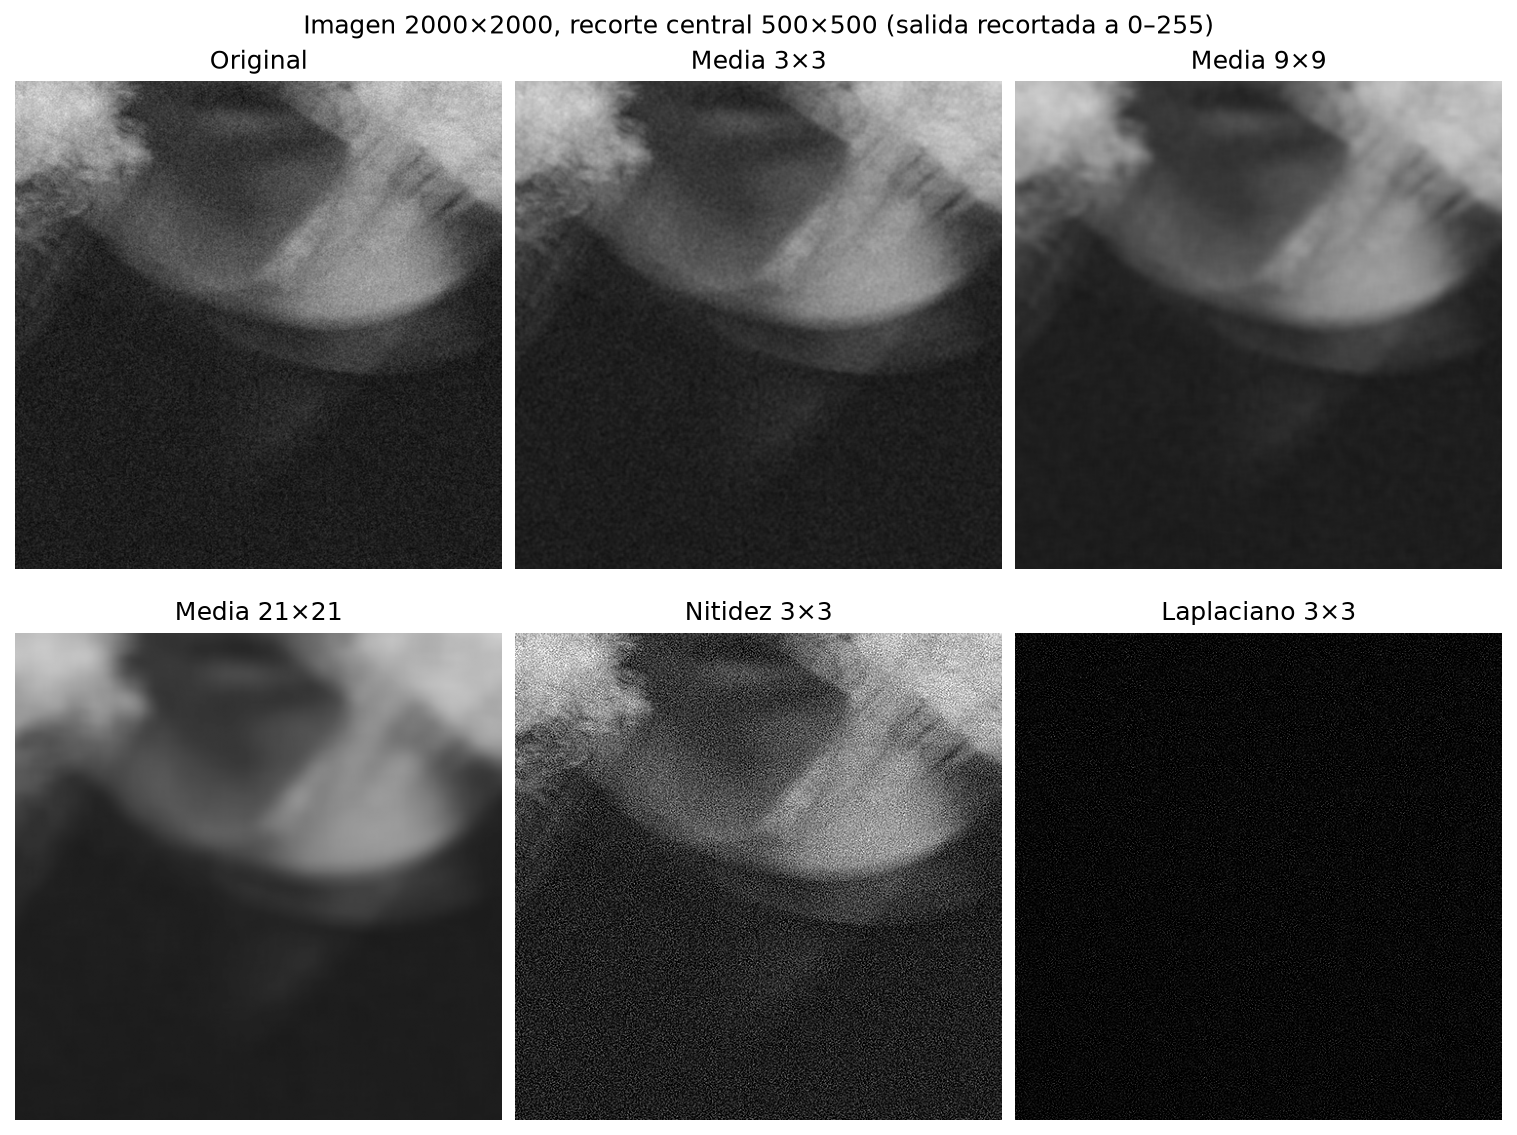
\includegraphics[width=0.85\textwidth]{figura_filtros_imagen.png}
\caption{Los filtros aplicados a la imagen de 2000 del experimento (recorte central de
$500\times500$).}
\end{figure}

\begin{table}[H]
\centering
\caption{Rango de la salida en \texttt{float} antes de pasar a $[0,255]$, imagen de 2000
(\texttt{resultados/rangos\_filtros.csv}).}\label{tab:rangos}
\begin{tabular}{lrrrr}
\toprule
Filtro & Mín. & Máx. & \% $<0$ & \% $>255$ \\
\midrule
Media $3\times3$ & 9.4 & 244.0 & 0 & 0 \\
Media $9\times9$ & 13.1 & 233.7 & 0 & 0 \\
Media $21\times21$ & 13.1 & 229.9 & 0 & 0 \\
Nitidez & $-91.0$ & 724.0 & 3.9 & 2.4 \\
Laplaciano & $-488.0$ & 114.0 & 49.0 & 0 \\
\bottomrule
\end{tabular}
\end{table}

La media nunca se sale de $[0,255]$, así que la conversión no le afecta. La nitidez se sale
por los dos lados en pocos píxeles, en los bordes más marcados, y ahí el recorte la satura. Con
el laplaciano casi la mitad de los píxeles quedan negativos y al recortarlos a 0 se vuelven
negros; por eso la imagen se ve casi toda negra y solo aparecen los bordes del lado positivo.
Es un efecto de la conversión y no del cálculo, que ya se validó antes. Los rangos los
calculamos aparte con \texttt{numpy} (\texttt{scripts/figuras\_filtros.py}) y coinciden con los
del programa.

\begin{figure}[H]
\centering
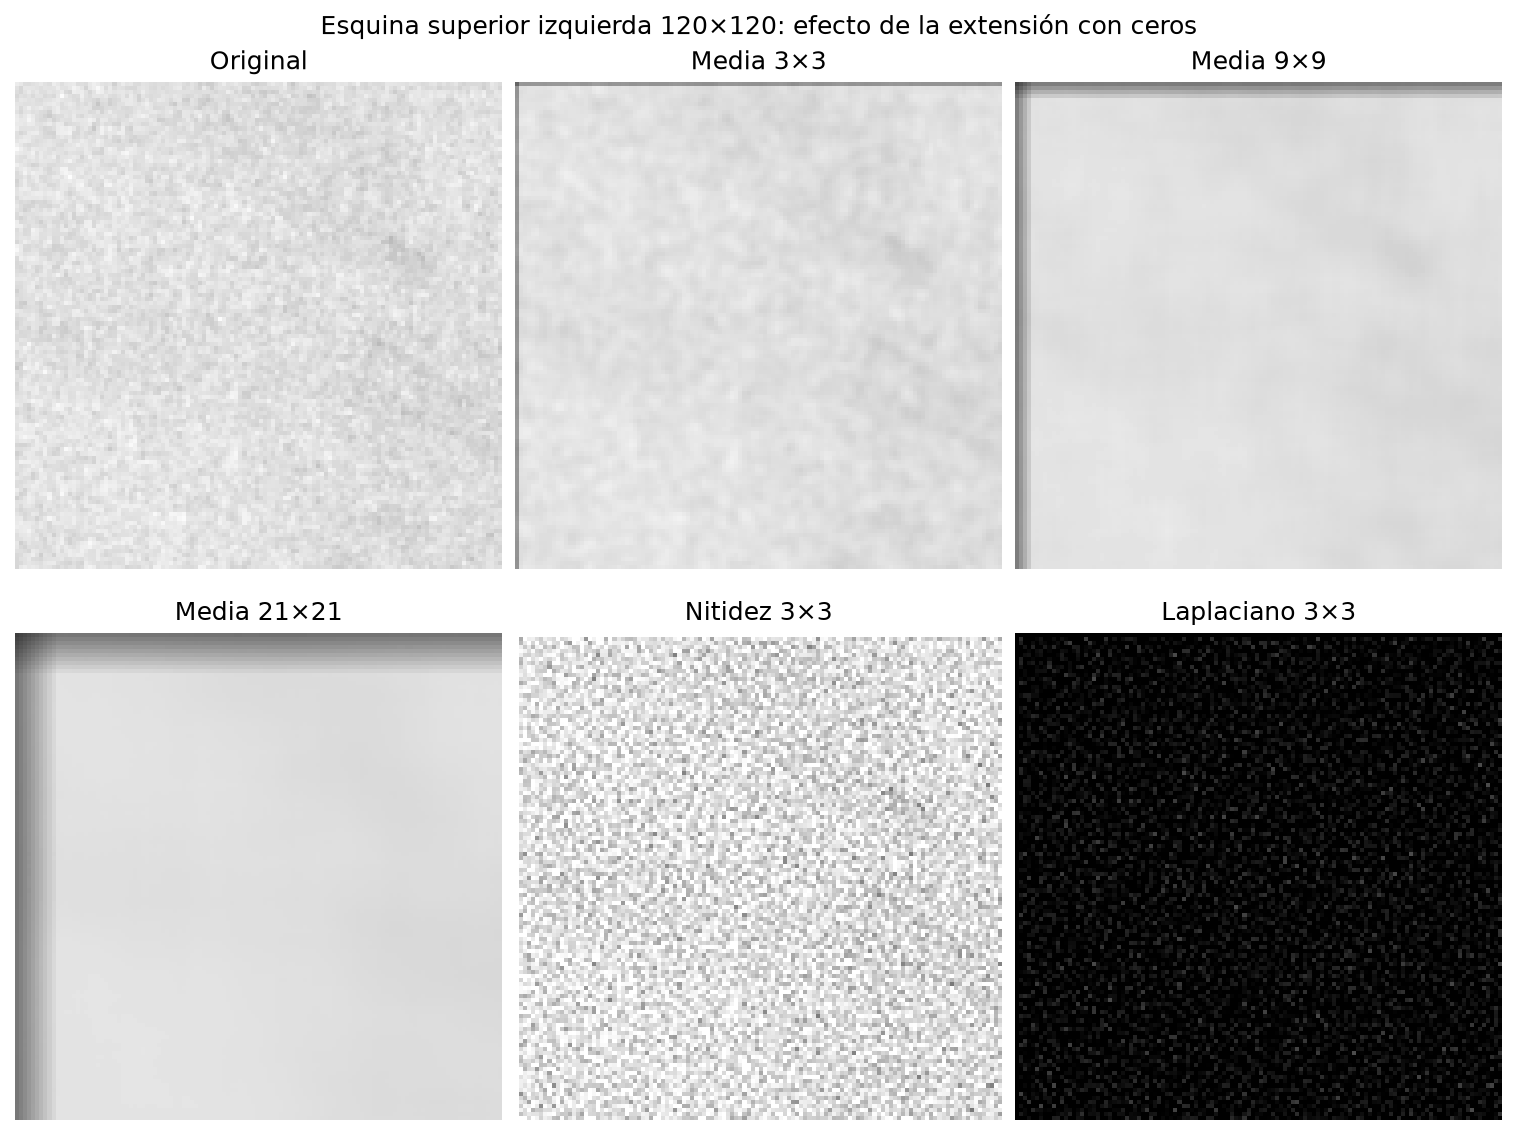
\includegraphics[width=0.65\textwidth]{figura_bordes.png}
\caption{Esquina de la imagen de 2000: con extensión con ceros aparece una franja oscura de
$\lfloor k/2\rfloor$ píxeles (1, 4 y 10 para $k=3,9,21$).}
\end{figure}

\section{Resultados}

Revisamos el registro de \texttt{nvidia-smi} (\texttt{resultados/gpu\_estado.csv}) con la hora
de cada bloque GPU que imprime el programa: las 12 configuraciones se midieron con la GPU en P0,
a 2535--2550\,MHz y con PCIe Gen~4. La temperatura estuvo entre 38 y 59\,$^\circ$C. Antes de empezar la GPU estaba en reposo
(P8, 210\,MHz, 3.3\,W) y Ollama, que usa la GPU en ese equipo, estuvo apagado durante toda la
medición.

Las mediciones son muy estables. La desviación del kernel es, en la mediana de las 12
configuraciones, el 0.04\,\% de su media (0.49\,\% en el peor caso); la del tiempo total GPU,
el 0.27\,\%, y la de la CPU, el 0.79\,\%. Las configuraciones que se repiten en varios
experimentos dan casi lo mismo: media $9\times9$ en 4000 con 256 hilos tarda 2.767, 2.780 y
2.780\,ms de kernel en los experimentos 2, 3 y 4.

\begin{table}[H]
\centering
\small
\caption{Medianas de 5 repeticiones. Tiempos en ms; $\sigma$: desviación estándar; Acel.:
aceleración de cómputo / con transferencias; \% transf.: porcentaje del tiempo GPU en copias
(mediana por repetición).}\label{tab:resultados}
\resizebox{\textwidth}{!}{\tabla{tabla_resumen.tex}}
\end{table}

\begin{figure}[H]
\centering
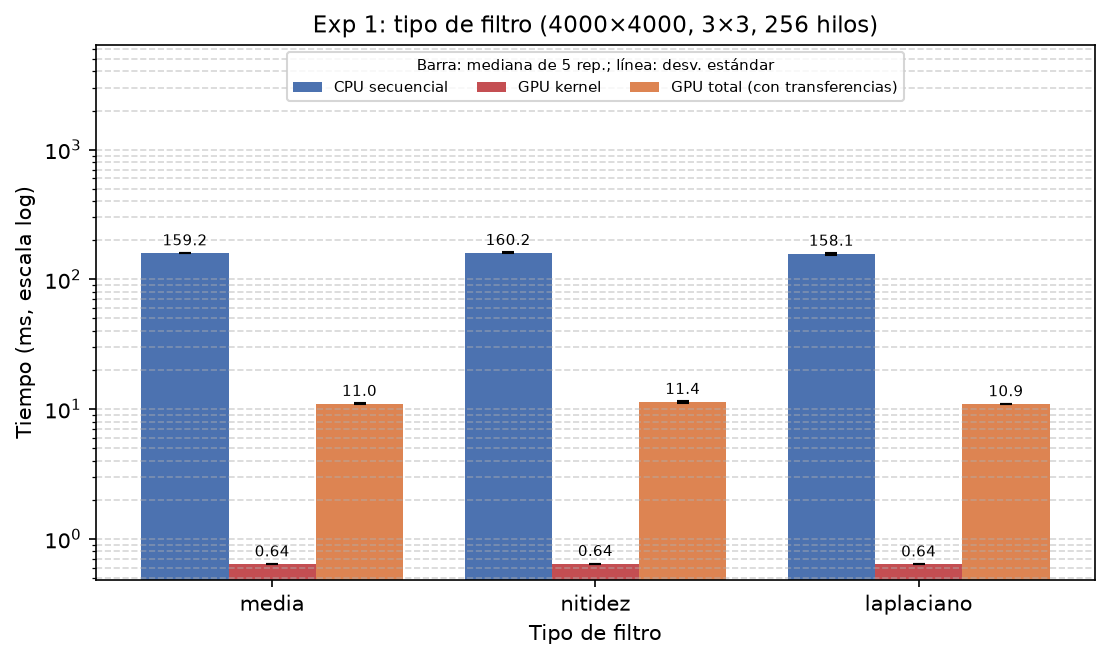
\includegraphics[width=0.49\textwidth]{grafica_exp1_filtros.png}
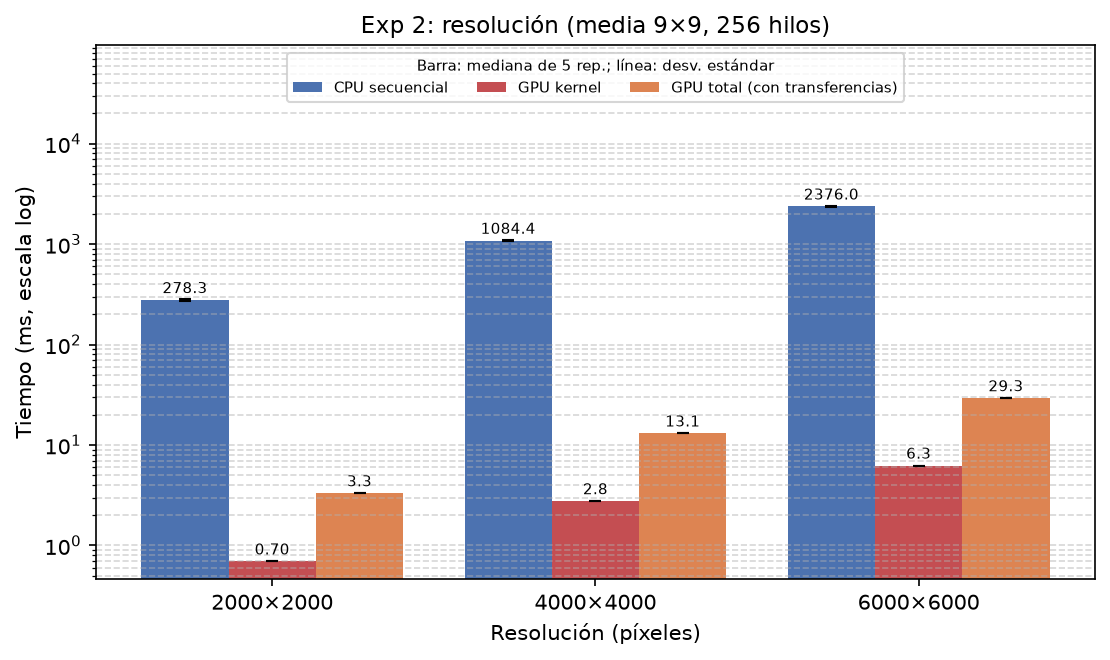
\includegraphics[width=0.49\textwidth]{grafica_exp2_resolucion.png}
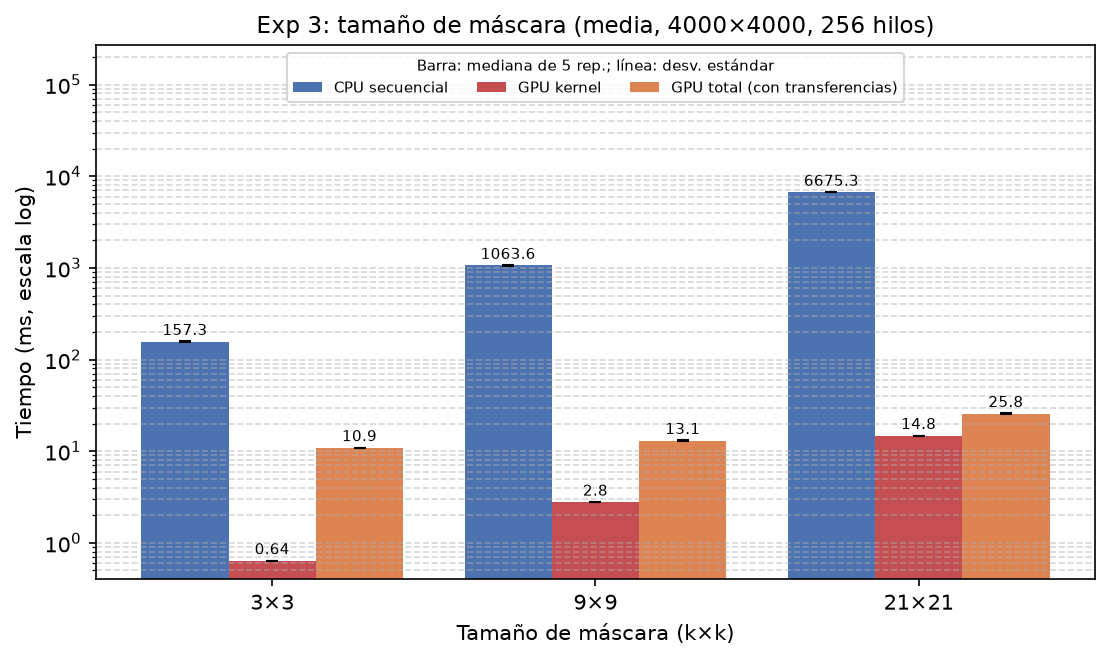
\includegraphics[width=0.49\textwidth]{grafica_exp3_mascara.png}
\caption{Tiempos de CPU, kernel y total GPU en los experimentos de filtro, resolución y
máscara.}\label{fig:experimentos}
\end{figure}

\begin{figure}[H]
\centering
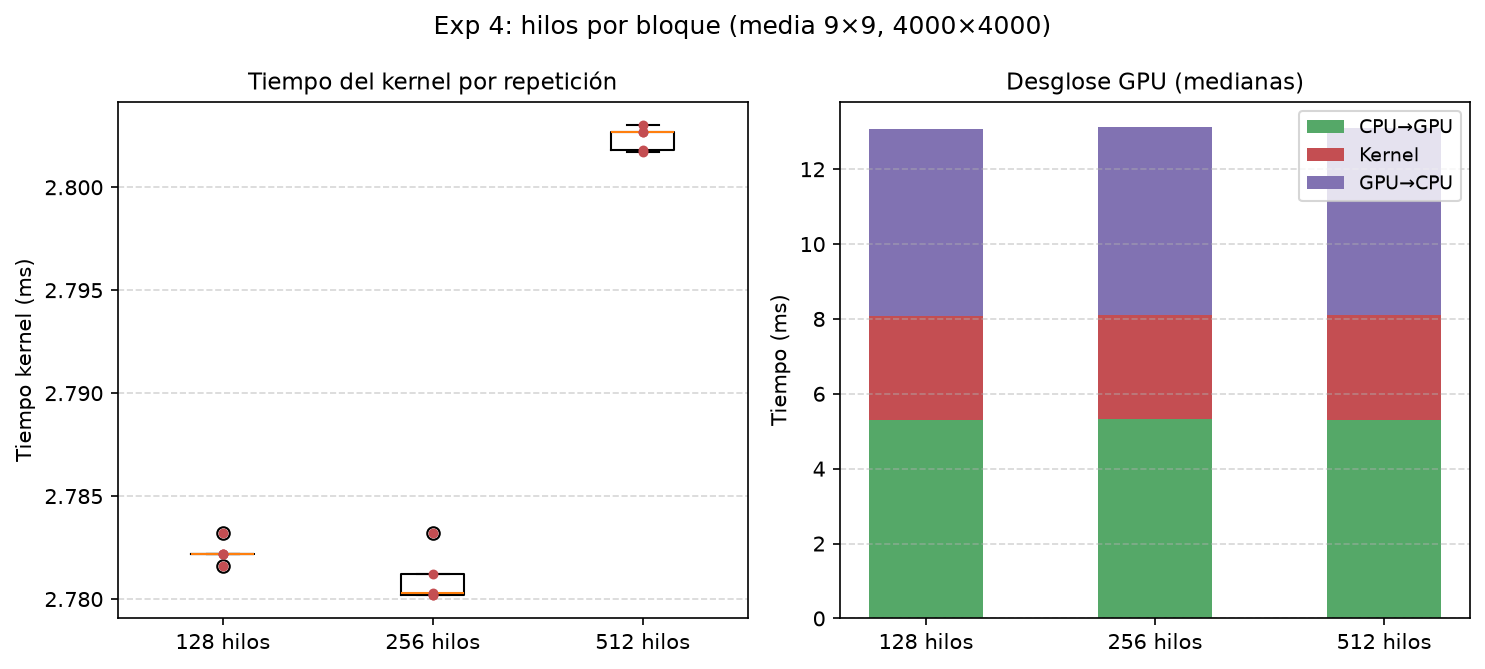
\includegraphics[width=0.9\textwidth]{grafica_exp4_hilos.png}
\caption{Kernel por repetición y reparto del tiempo GPU según los hilos por bloque.}\label{fig:hilos}
\end{figure}

\begin{figure}[H]
\centering
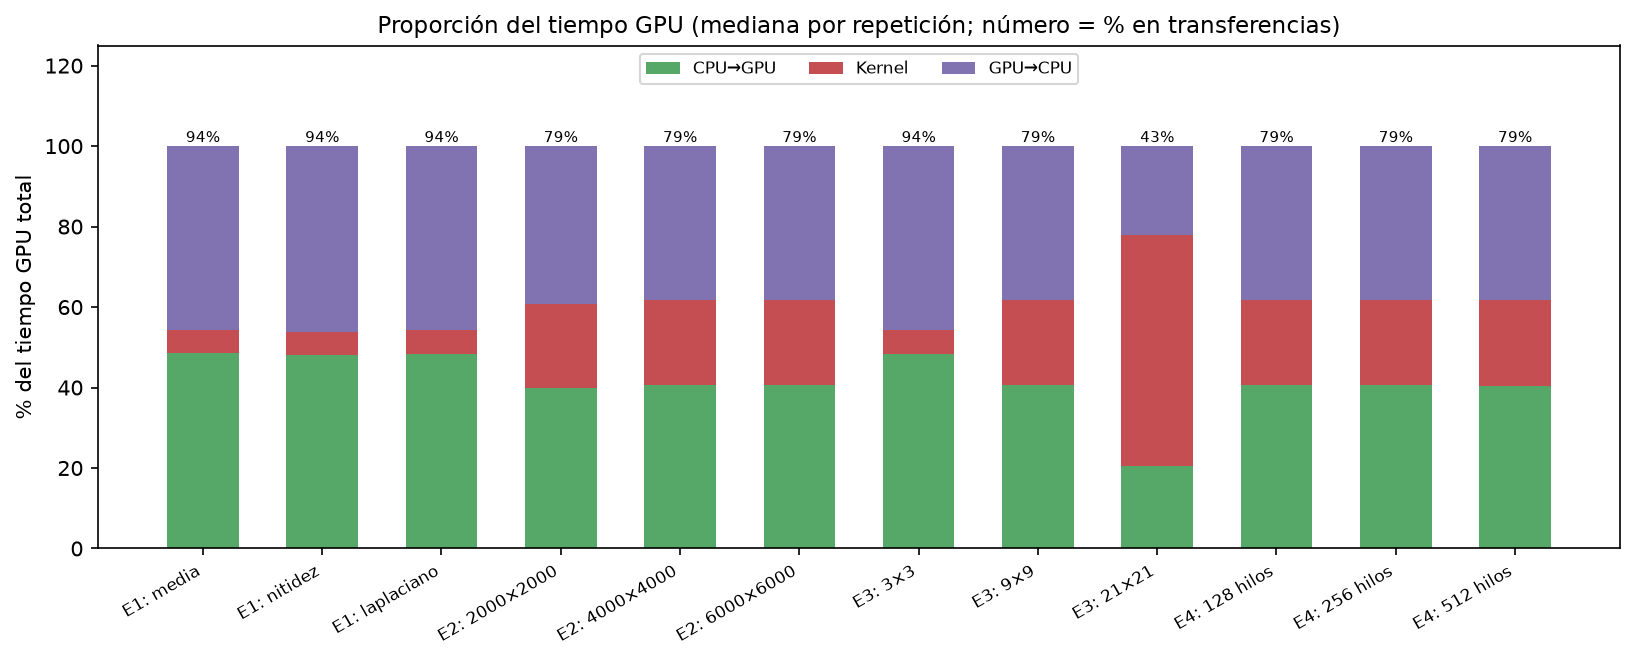
\includegraphics[width=\textwidth]{grafica_gpu_desglose.png}
\caption{Reparto del tiempo GPU entre copias y kernel.}\label{fig:desglose}
\end{figure}

\begin{figure}[H]
\centering
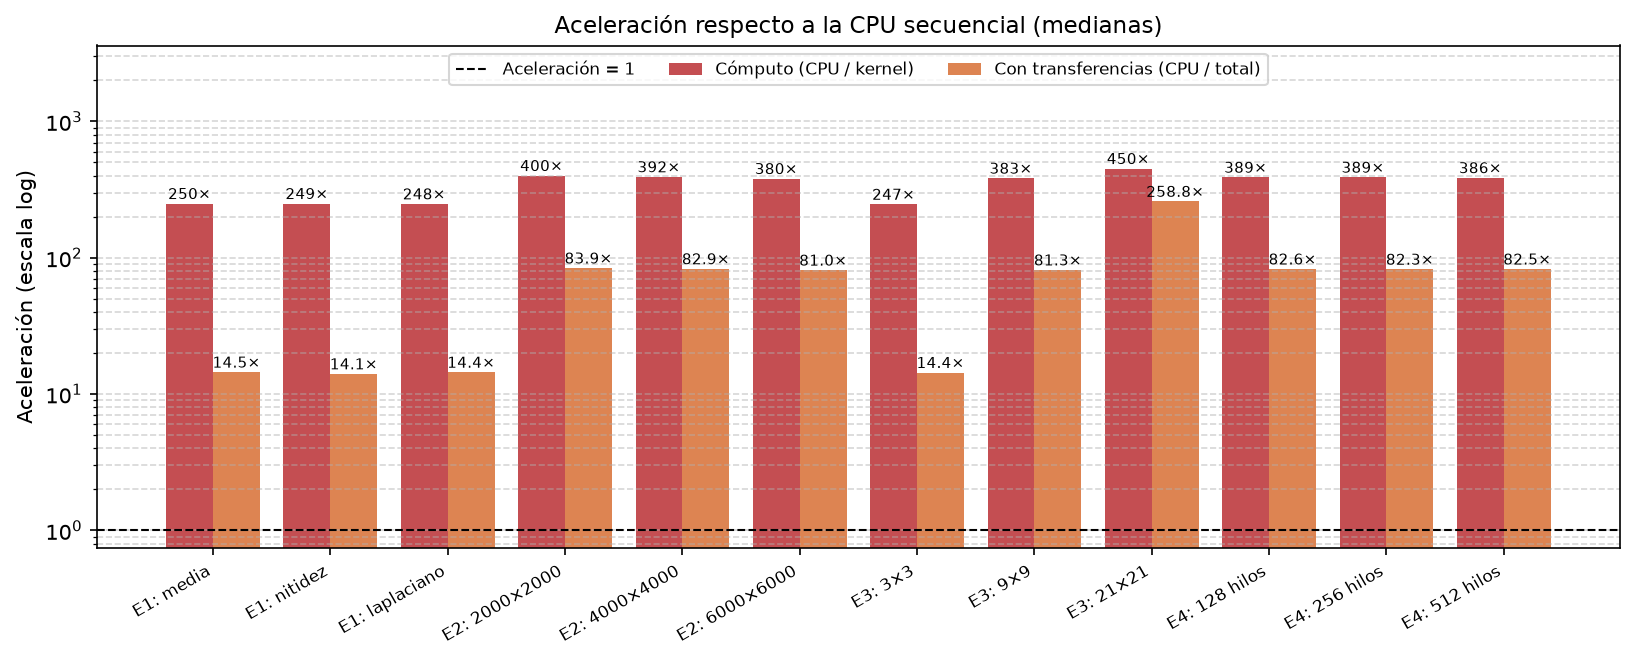
\includegraphics[width=\textwidth]{grafica_speedup.png}
\caption{Aceleración de cómputo y con transferencias.}\label{fig:aceleracion}
\end{figure}

\section{Análisis}

\subsection{¿Cómo cambia el tiempo con la resolución y el tamaño de la máscara?}

En la CPU el trabajo es de $n\cdot k^2$ multiplicaciones y sumas, y el tiempo lo sigue de cerca.
Con media $9\times9$ pasa de 278.3 a 1084.4 y a 2376.0\,ms para 2000, 4000 y 6000: con 4 y 9
veces más píxeles crece 3.9 y 8.5 veces. En la imagen de 4000 la máscara lo lleva de 157.3 a
1063.6 y a 6675.3\,ms para $k=3$, 9 y 21; ahí $k^2$ crece 9 y 49 veces y el tiempo 6.8 y 42.4.
Cada producto cuesta entre 0.82 y 1.11\,ns. Con $3\times3$ sale un poco más caro, seguramente
porque recorrer la imagen y escribir la salida pesa más cuando solo hay 9 productos por píxel.

En la GPU hay que separar copias y kernel. Las copias solo dependen de la resolución: la de
CPU$\to$GPU tarda 1.32, 5.31 y 11.89\,ms, crece igual que los píxeles y con las tres máscaras
se queda en 5.30\,ms. El kernel también crece como $n$ (0.695, 2.767 y 6.250\,ms), pero con la
máscara no se comporta igual en todo el rango. De $3\times3$ a $9\times9$ hay 9 veces más
productos y el kernel solo tarda 4.4 veces más (de 0.638 a 2.780\,ms); de $9\times9$ a
$21\times21$ hay 5.4 veces más y tarda 5.3 veces más (14.82\,ms). Por producto, el kernel tarda
0.0044\,ns con $3\times3$ y 0.0021\,ns con las máscaras más grandes. Nuestra explicación es que
con $3\times3$ hay tan poco cálculo que manda el acceso a memoria: leer y escribir 64\,MB cada
uno en 0.638\,ms equivale a unos 200\,GB/s. No lo comprobamos con un perfilador.

El tipo de filtro no cambia el tiempo si la máscara es del mismo tamaño. En la CPU, media,
nitidez y laplaciano tardan 159.2, 160.2 y 158.1\,ms, y en la GPU 0.638, 0.642 y 0.637\,ms; las
diferencias son del orden de la variación entre repeticiones.

\subsection{¿Qué proporción del tiempo GPU corresponde a transferencias?}

Mucha, salvo con la máscara grande. Calculando el porcentaje en cada repetición, las copias
son entre el 94.2 y el 94.5\,\% del tiempo GPU con $3\times3$, entre el 78.6 y el 79.2\,\% con
$9\times9$ (en las tres resoluciones y con los tres valores de hilos) y entre el 41.3 y el
43.4\,\% con $21\times21$ (figura~\ref{fig:desglose}). Con la resolución el porcentaje no se
mueve porque copias y kernel crecen al mismo ritmo. Con la máscara baja, porque se copia lo
mismo y el kernel tiene más trabajo. Solo con $21\times21$ el kernel tarda más que las dos
copias juntas (14.82 frente a 10.97\,ms).

\subsection{Aceleración}

La aceleración de cómputo es de unas 250 veces con $3\times3$, entre 380 y 400 con $9\times9$ y
450 con $21\times21$. Sube con $k$, probablemente porque con $3\times3$ el kernel está limitado
por la memoria y no aprovecha toda la capacidad de cálculo de la GPU. Con la resolución baja un
poco (400, 392 y 380) porque la CPU se vuelve algo más eficiente por producto en las imágenes
grandes (de 0.86 a 0.82\,ns), mientras el kernel se mantiene en 0.0021\,ns.

Cuando se suman las copias el panorama cambia: unas 14 veces con $3\times3$, entre 81 y 84 con
$9\times9$ y 259 con $21\times21$ (figura~\ref{fig:aceleracion}). Con $3\times3$ las copias se
llevan casi toda la ganancia y la aceleración cae unas 17 veces; con $21\times21$ cae menos de
la mitad. En este equipo, mandar a la GPU un solo filtro pequeño sobre una imagen que está en
la memoria de la CPU aprovecha poco la GPU; cuanto más trabajo hay por píxel, más compensa.

\subsection{¿Qué configuración de hilos por bloque es mejor y qué variabilidad presenta?}

Con 128, 256 y 512 hilos el kernel tarda 2.782, 2.780 y 2.803\,ms de mediana, con desviaciones
de 0.0006, 0.0013 y 0.0006\,ms y rangos de 2.7816--2.7832, 2.7802--2.7832 y 2.8017--2.8030\,ms.
128 y 256 son prácticamente iguales: sus rangos se cruzan. Con 512 el kernel es un 0.8\,\% más
lento, unos 22\,$\mu$s, y como sus cinco repeticiones quedan por encima de todas las demás, la
diferencia es real aunque pequeña. En el tiempo total no se nota (13.09, 13.14 y 13.10\,ms)
porque lo dominan las copias. La mejor mediana es la de 256 hilos, empatada en la práctica con
128. No sabemos por qué 512 es algo más lento; podría tener que ver con la ocupación de los
multiprocesadores o con cómo se reparten los bloques, pero habría que comprobarlo con un
perfilador como Nsight Compute.

\subsection{¿Qué confirma o contradice las expectativas?}

Esperábamos que el tiempo de la CPU fuera proporcional a $n\cdot k^2$, que el tipo de filtro no
influyera con una máscara del mismo tamaño y que la GPU diera el mismo resultado que la CPU;
las tres cosas se cumplieron. También esperábamos que las copias crecieran con $n$ y no
dependieran de $k$, y que pesaran mucho con máscaras pequeñas: con $3\times3$ la aceleración
pasa de unas 250 veces a unas 14 al incluirlas.

Lo que no salió como esperábamos fue el kernel con máscaras pequeñas. Suponíamos que crecería
como $k^2$ y de $3\times3$ a $9\times9$ creció menos de la mitad de lo previsto, lo que apunta
a que con $3\times3$ el límite es la memoria y no el cálculo. Con los hilos por bloque
esperábamos diferencias pequeñas, porque 128, 256 y 512 son múltiplos de 32, el tamaño de un
warp \cite{cudaguide}, y así fue: la mayor es de 0.8\,\%.

Tampoco esperábamos que la gestión de energía de la GPU portátil influyera tanto. Sin un
calentamiento largo, la misma configuración varió hasta 8 veces (sección~\ref{sec:metodologia});
con el protocolo final la variación del kernel bajó a 0.04\,\%. La copia CPU$\to$GPU llega a
11.5--12.2\,GB/s con el enlace en Gen~4, aunque copiar desde memoria paginable obliga al
driver a pasar por un búfer intermedio \cite{cudaguide}; no probamos con memoria fija
(\texttt{cudaMallocHost}).

\section{Limitaciones}

Todo se midió en un solo portátil y con las configuraciones de la tabla, así que las
conclusiones no se pueden extender a otras GPU o tamaños. La GPU tiene gestión de energía y no
fijamos sus frecuencias; lo compensamos con el calentamiento y comprobamos con
\texttt{nvidia-smi} que todas las mediciones se hicieron en P0. Las aceleraciones comparan la
versión secuencial, que usa un solo núcleo de la CPU, con toda la GPU, no con una versión
paralela en CPU. Con 5 repeticiones la mediana es confiable, pero la desviación estándar es
poco precisa. El tiempo total no incluye la reserva de memoria y el host usa memoria paginable.
El kernel es básico: trabaja en memoria global, sin memoria compartida ni constante, y lee la
máscara de memoria global en cada producto. Por último, convertir a $[0,255]$ recortando
esconde la mitad negativa del laplaciano.

\section{Conclusiones}

Las versiones en CPU y CUDA dan el mismo resultado: el error es 0 con coeficientes enteros y
como mucho $1.22\times10^{-4}$ con la media, por debajo de la tolerancia de $10^{-3}$.

En la CPU el tiempo crece en proporción a $n\cdot k^2$. En la GPU las copias crecen con la
resolución y no dependen de la máscara, y el kernel crece con $n$ y, desde $9\times9$, con
$k^2$; con $3\times3$ parece limitado por el acceso a memoria.

Las copias se llevan la mayor parte del tiempo GPU con máscaras pequeñas (94\,\% con
$3\times3$ y 79\,\% con $9\times9$) y solo con $21\times21$ domina el cálculo. Por eso la
aceleración de cómputo, de 250 a 450 veces, se queda en 14, 82 y 259 veces cuando se incluyen
las copias: lo que se gana de verdad depende del trabajo por píxel.

Los hilos por bloque casi no influyen. 256 y 128 dan lo mismo y 512 es un 0.8\,\% más lento.

En una GPU portátil hay que calentar antes de medir. Sin hacerlo, la misma configuración varió
hasta 8 veces; con 2\,s de calentamiento y las repeticiones seguidas, la variación del kernel
bajó a 0.04\,\%.

Estas conclusiones valen para este equipo y las configuraciones que probamos.

\section{Contribuciones}

\begin{table}[H]
\centering
\caption{Contribuciones de los integrantes.}
\begin{tabular}{lp{11cm}}
\toprule
Integrante & Contribución \\
\midrule
Michael Lata (Bloque 1) & Lectura y escritura PGM, máscaras, convolución secuencial, prueba
  manual, preparación de imágenes, datos del equipo y ejecución de las mediciones en su
  portátil. \\
Jordi Romero (Bloque 2) & Kernel CUDA, reserva y copias CPU--GPU, medición con eventos CUDA y
  validación CPU vs GPU con la imagen de $1001\times777$. \\
Andres Morocho (Bloque 3) & Diseño de los experimentos y del protocolo de medición, CSV,
  validación por configuración, estadística, gráficas, figuras de filtros, informe y
  presentación. \\
\bottomrule
\end{tabular}
\end{table}

\section{Reproducibilidad}

Repositorio: \repo, commit \texttt{b5a199e}.

\begin{lstlisting}[language=bash]
cmake -S . -B build && cmake --build build -j
python3 scripts/preparar_imagenes.py datos/original.jpg
./build/convolucion probar          # prueba manual y validación GPU
./build/convolucion medir           # resultados/mediciones.csv
python3 scripts/graficas.py         # tabla y gráficas
python3 scripts/figuras_filtros.py  # imágenes de los filtros y rangos
\end{lstlisting}

\section*{Firmas}
\addcontentsline{toc}{section}{Firmas}
\vspace{2cm}
\noindent
\begin{tabular}{ccc}
\rule{4.3cm}{0.4pt} & \rule{4.3cm}{0.4pt} & \rule{4.3cm}{0.4pt} \\
Michael Lata & Jordi Romero & Andres Morocho \\
\end{tabular}

%%%%%%%%%%%%%%%%%%%%%%%%%%%%%%%%%%%%%%%%%%%%%%%%%%%%%%%%%%%%%%%%%%%%%%%%%%%%%%%%%%%%%%%%%
%%%%%%%%%%%%%     FIN   TEXTO     %%%%%%%%%%%%%%%%%%%%%%%%%%%%%%%%%%%%%%%%%%%%%%%%%%%%%%%
%%%%%%%%%%%%%%%%%%%%%%%%%%%%%%%%%%%%%%%%%%%%%%%%%%%%%%%%%%%%%%%%%%%%%%%%%%%%%%%%%%%%%%%%%

\newpage
\bibliographystyle{plain}
\bibliography{biblist}

\end{document}
